\documentclass{article}
\usepackage{a4wide}


\usepackage{polski}
\usepackage[utf8x]{inputenc}
\usepackage{graphicx}
\usepackage{float}
\usepackage{hyperref}
\usepackage{listings}
\usepackage{mathtools}
\usepackage{amsmath}
\usepackage{amssymb}

\usepackage{color} %red, green, blue, yellow, cyan, magenta, black, white
\definecolor{mygreen}{RGB}{28,172,0} % color values Red, Green, Blue
\definecolor{taupe}{rgb}{0.28, 0.24, 0.2}
\definecolor{mylilas}{RGB}{0,110,0}


\author{Lev Sergeyev}
\title{SPC. Ćwiczenie 6. Systemy o złożonej strukturze. Sterowanie optymalne, wielowarstwowe}

\date{20.12.2019, pt/TN 13:15}
\begin{document}

\maketitle

%\pagebreak


\section{Liniowy system statyczny o złożonej strukturze}
\par
Zaprojektowano model systemu statycznego o złożonej strukturze:

\begin{equation}
Y = K U = (\mathbf{I} - A H)^{-1} B U
\end{equation}

\begin{figure}[h]
\centering
\scalebox{0.4}{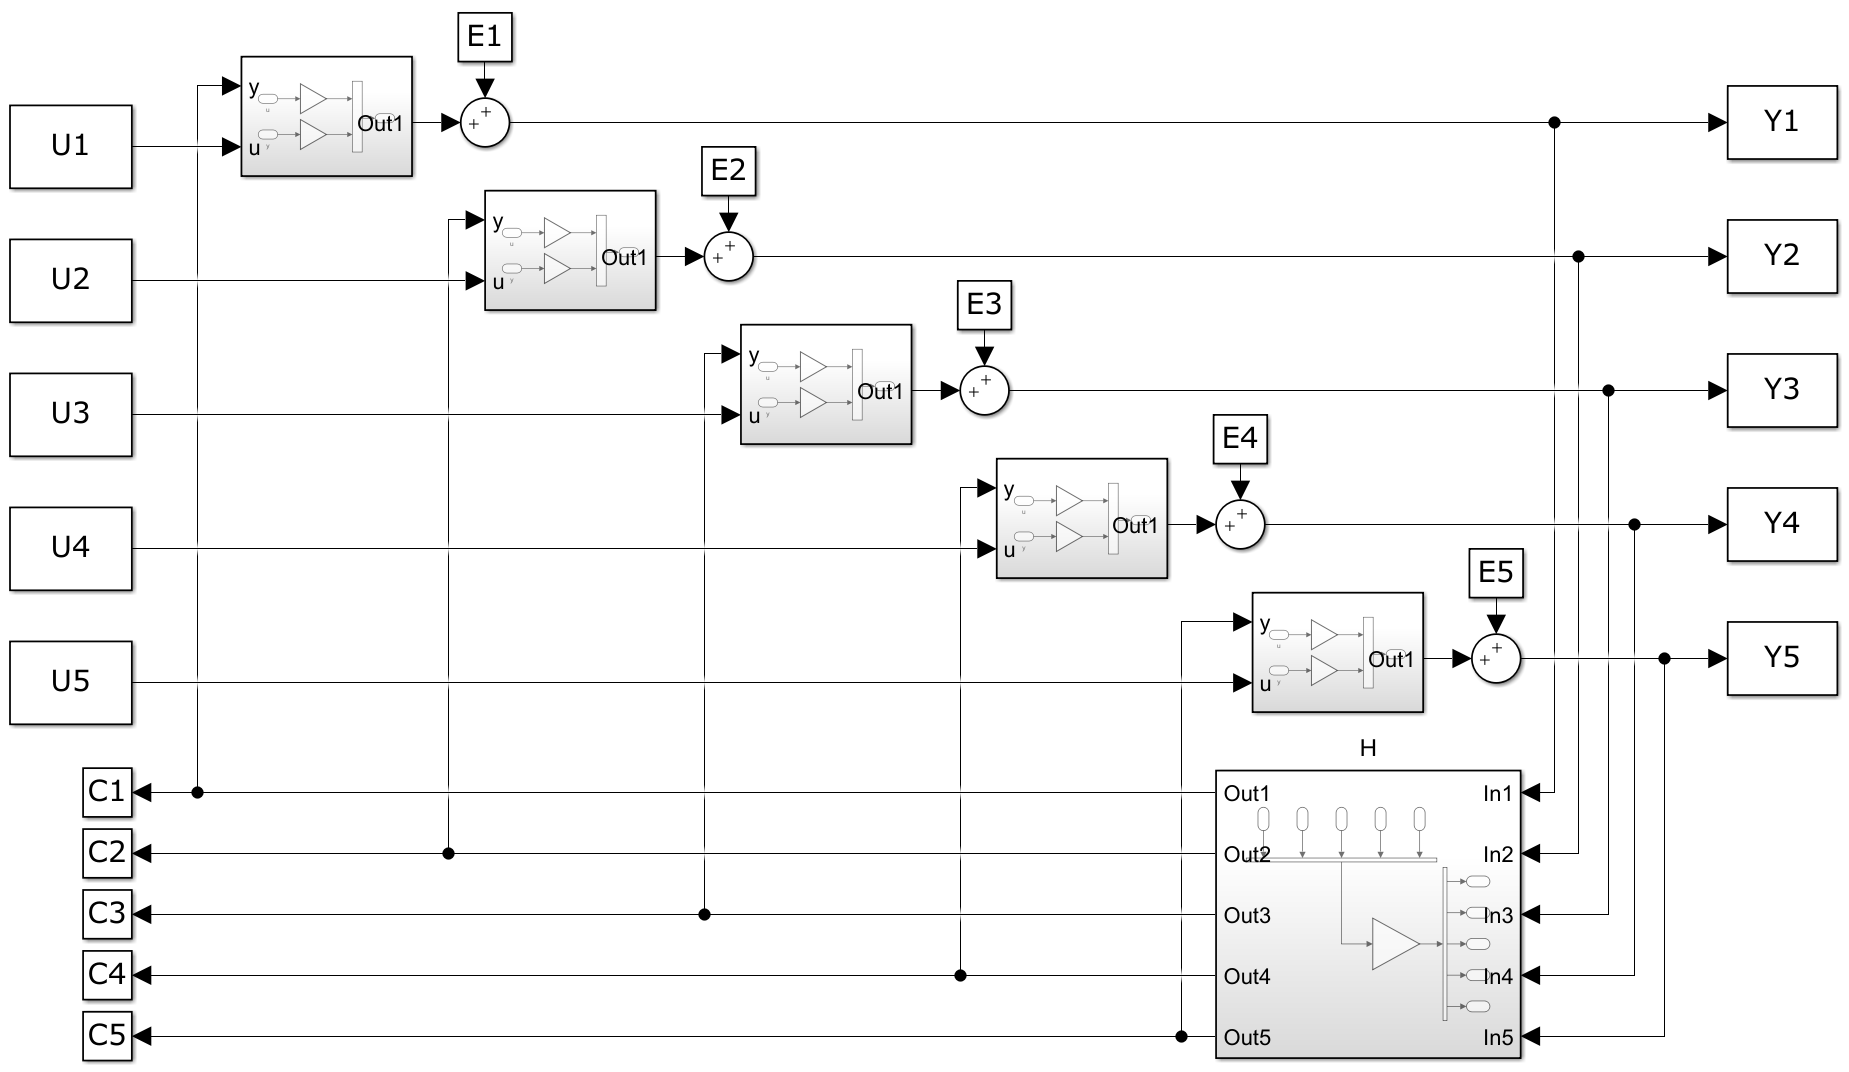
\includegraphics{model.png}}
\caption{Model systemu}
\end{figure}

Parametry systemu:
\begin{equation}
A = \begin{bmatrix}
1 & 0 & 0 & 0 & 0\\
0 & 1 & 0 & 0 & 0\\
0 & 0 & 1 & 0 & 0\\
0 & 0 & 0 & 1.3 & 0\\
0 & 0 & 0 & 0 & 0.5\\
\end{bmatrix}
,
B = \begin{bmatrix}
2 & 0 & 0 & 0 & 0\\
0 & 3 & 0 & 0 & 0\\
0 & 0 & 2 & 0 & 0\\
0 & 0 & 0 & 2 & 0\\
0 & 0 & 0 & 0 & 2\\
\end{bmatrix}
,
H = \begin{bmatrix}
0 & 0 & 0 & 0 & 1\\
1 & 0 & 0 & 0 & 0\\
0 & 1 & 0 & 0 & 0\\
0 & 0 & 1 & 0 & 0\\
0 & 0 & 0 & 1 & 0\\
\end{bmatrix}
\end{equation}

\begin{figure}[ht]
\centering
\scalebox{0.35}{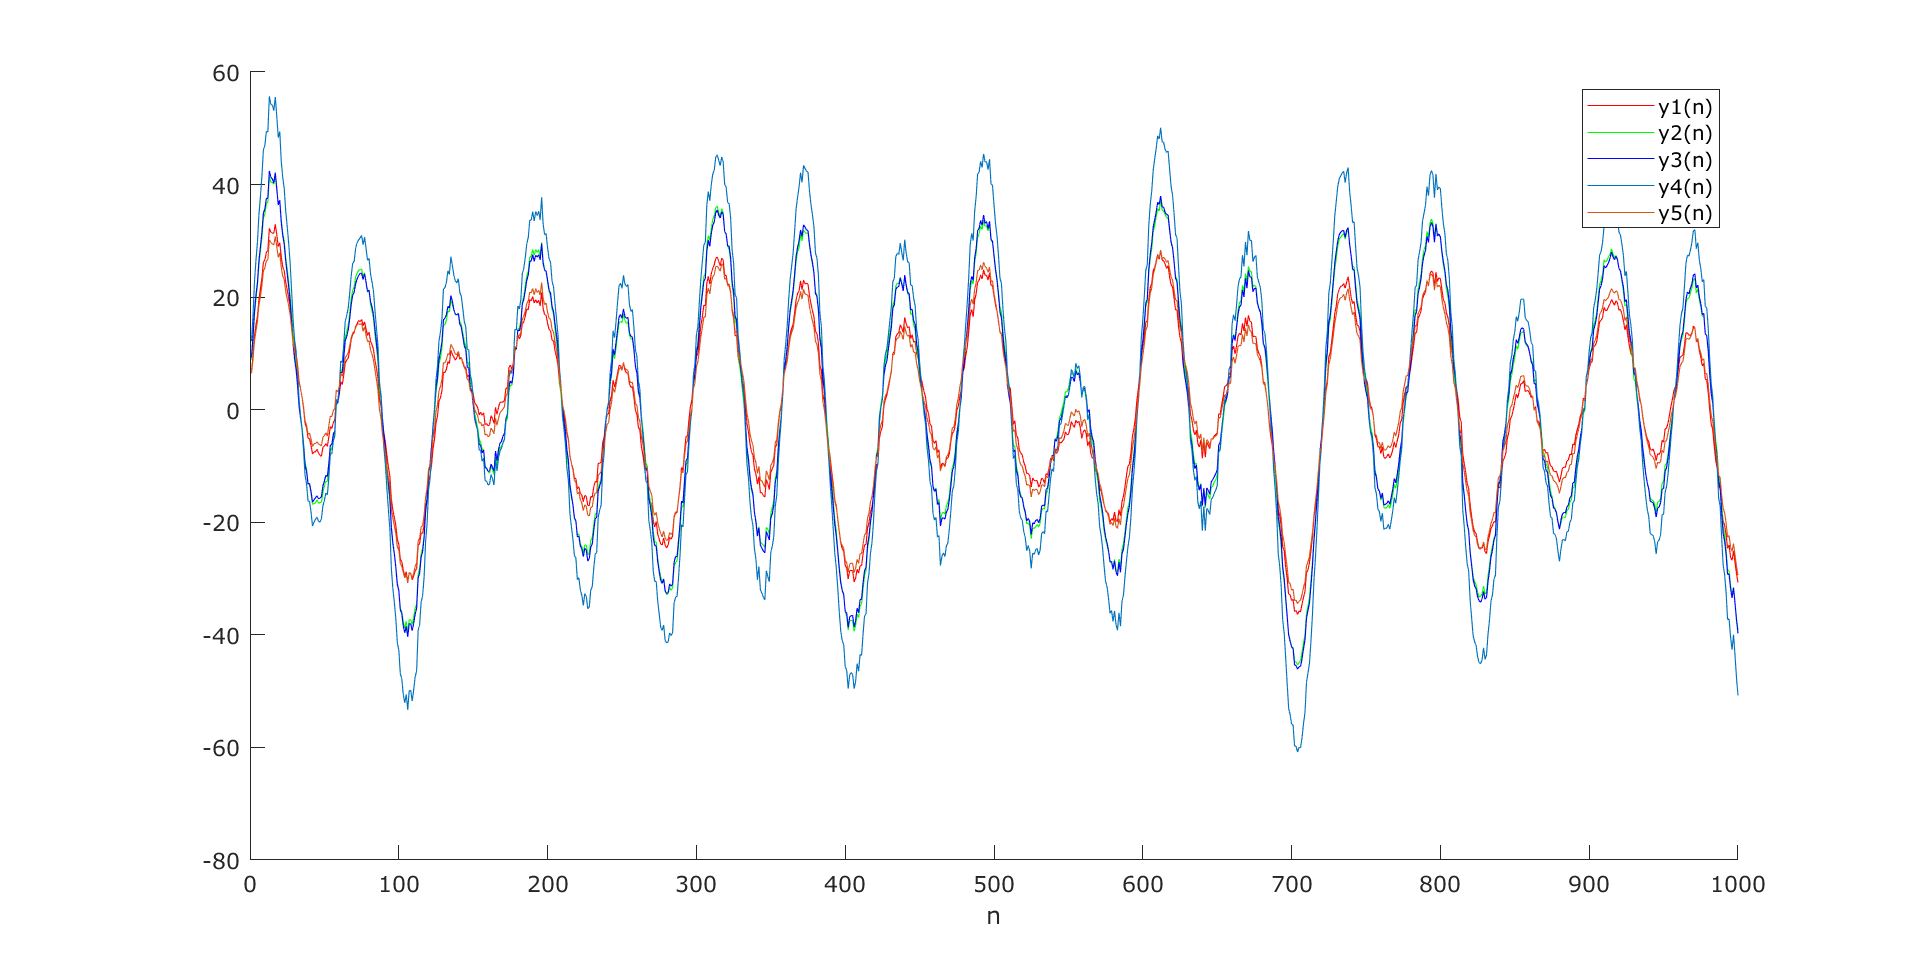
\includegraphics{sym.png}}
\caption{Odpowiedź na wymuszenie sinusoidalne}
\end{figure}

%\pagebreak

\section{Identyfikowalność}

Tw.  
\begin{equation}
rank \hspace{2pt}H_i
A = \begin{bmatrix}
K_1 & \cdots & K_{i-1} & K_{i+1} & \cdots & K_N
\end{bmatrix}
 = dim \hspace{2pt} u_i 
\end{equation}
pozwala na określenie identyfikowalności systemu. \\
Dla danego systemu, wszystkie równości:
\begin{equation}
rank \hspace{2pt}H_i (\mathbf{I} - A H)^{-1} diag [B_1 \cdots B_{i-1} \hspace{3pt} 0 \hspace{3pt} B_{i+1} \cdots B_n] = dim \hspace{2pt} u_i 
\end{equation}
są prawdziwe. System jest identyfikowalny

\section{Identyfikacja}

Używając metody NK rzeprowadzono identyfikację systemu w obecności zakłóceń losowych:

\begin{equation}
\Phi_N = \begin{bmatrix}
C_{N} & U_N
\end{bmatrix}
 = \begin{bmatrix}
c_0 & u_0 \\ 
c_1 & u_1 \\ 
\vdots & \vdots \\ 
c_n & u_n
\end{bmatrix}
\end{equation}

\begin{equation}
\widehat{\Theta} = (\Phi_N^T \Phi_N)^{-1} \Phi_N^T Y_N = \begin{bmatrix}
a \\  b
\end{bmatrix}
\end{equation}

\begin{equation}
\widehat{\Theta}_1 = \begin{bmatrix}
1.0005 \\ 1.9855
\end{bmatrix}
,
\widehat{\Theta}_2 = \begin{bmatrix}
1.0091 \\ 2.9368
\end{bmatrix}
,
\widehat{\Theta}_3 = \begin{bmatrix}
1.0001 \\ 1.9605
\end{bmatrix}
,
\widehat{\Theta}_4 = \begin{bmatrix}
1.3 \\ 1.9789
\end{bmatrix}
,
\widehat{\Theta}_5 = \begin{bmatrix}
0.5003 \\ 1.9992
\end{bmatrix}
\end{equation}

\section{Sterowanie}
Założono, wyjście żądane przyjmuje następujące wartości:
\begin{equation}
Y_{z} = \begin{bmatrix}
y_{z1} \\ y_{z2} \\ y_{z3} \\ y_{z4} \\ y_{z5}
\end{bmatrix}
= \begin{bmatrix}
5 \\ 4 \\ 3 \\ 2 \\ 1
\end{bmatrix}
\end{equation}
Wysterować \(U\) tak, aby ośiągnoć:
\begin{equation}
Q(u_1,u_2,u_3,u_4,u_5) = (y_1 - y_{z1})^2 + (y_2 - y_{z2})^2 + \cdots + (y_5 - y_{z5})^2 ) \rightarrow min
\end{equation}

\subsection{Sterowanie bez ograniczeń}
\begin{equation}
U_{opt} = K^{-1} Y = ((\mathbf{I} - A H)^{-1} B) ^ {-1} Y = B^{-1}(\mathbf{I} - A H) Y = \begin{bmatrix}
2 \\ -1/3 \\ -0.5 \\ -0.95 \\ 0
\end{bmatrix}
\end{equation}

\begin{figure}[ht]
\centering
\scalebox{0.35}{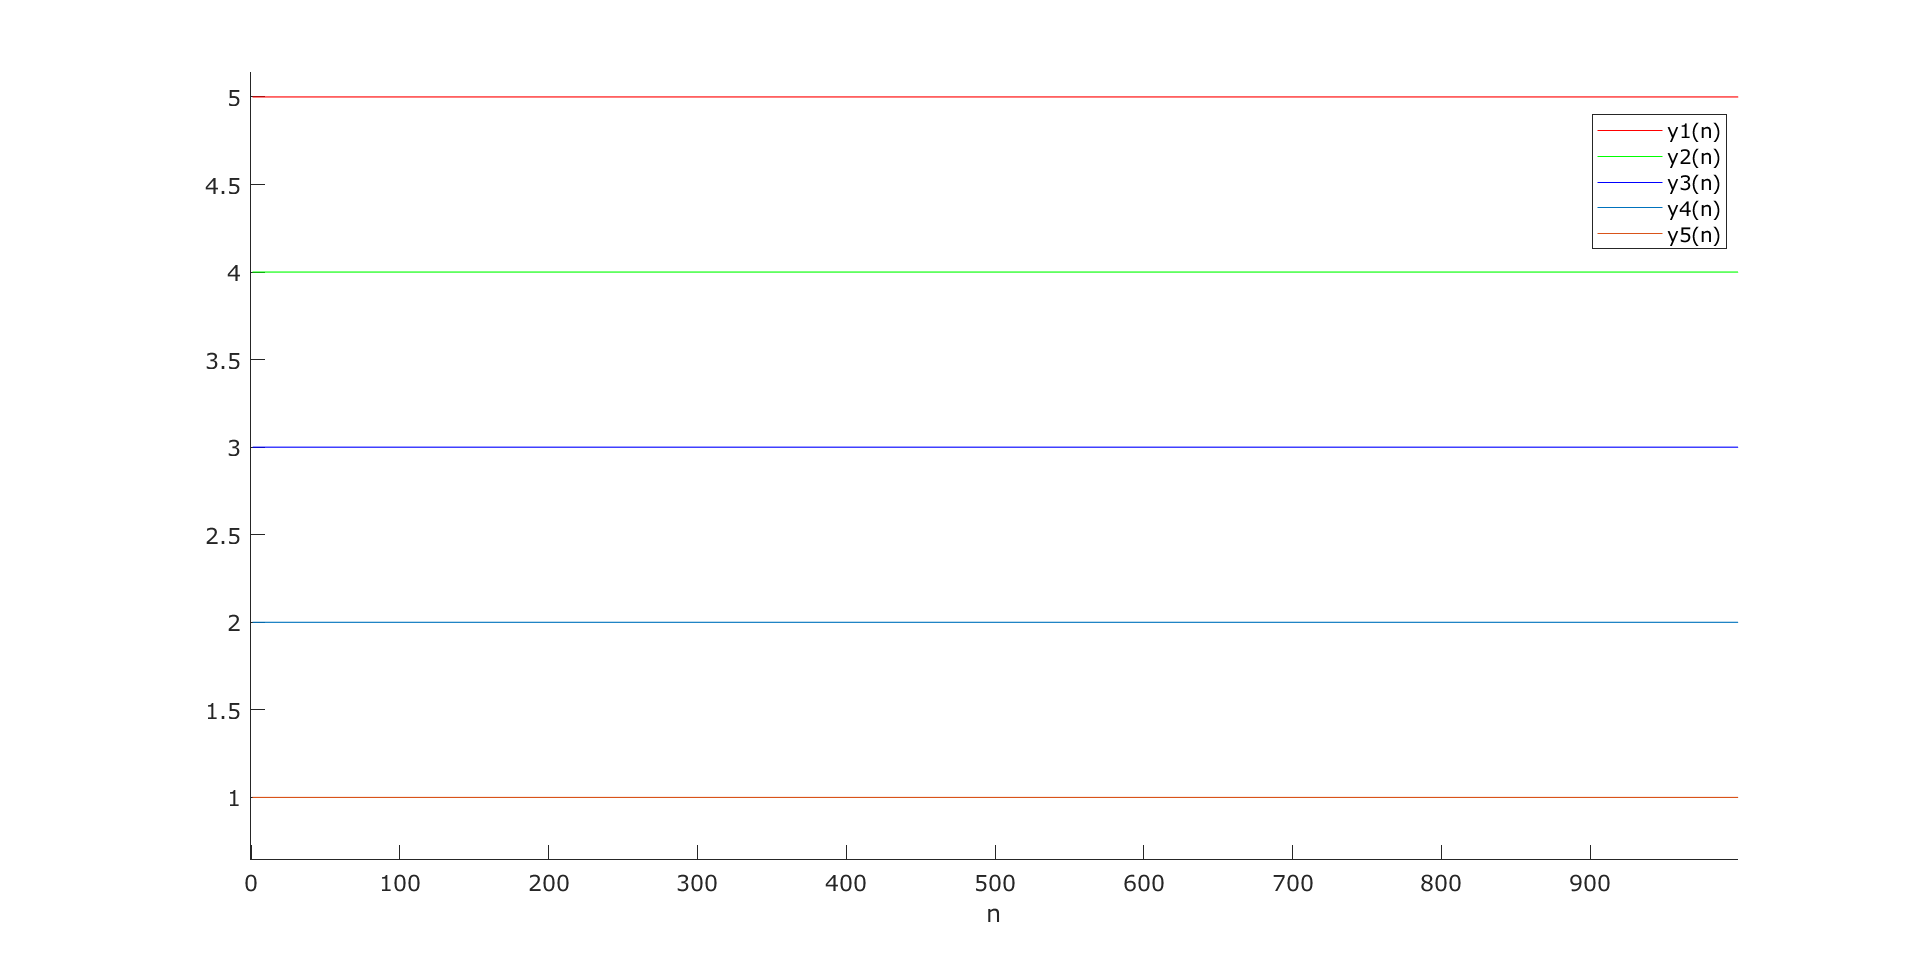
\includegraphics{s1.png}}
\caption{Sterowanie bez ograniczeń}
\end{figure}

\subsection{Sterowanie z ograniczeniami}
Wprowadzono ograniczenie:
\begin{equation}
u_1^2+u_2^2+u_3^2+u_4^2+u_5^2 \leqslant r
\end{equation}
Przejście na współrzędne sferyczne V wymiaru:
\begin{equation}
\begin{matrix}
u_1 = p \hspace{3pt} cos{\alpha} \\
u_2 = p \hspace{3pt} sin{\alpha} \hspace{3pt} cos{\beta} \\
u_2 = p \hspace{3pt} sin{\alpha} \hspace{3pt} sin{\beta} \hspace{3pt} cos{\gamma} \\
u_2 = p \hspace{3pt} sin{\alpha} \hspace{3pt} sin{\beta} \hspace{3pt} sin{\gamma} \hspace{3pt} cos{\theta} \\
u_2 = p \hspace{3pt} sin{\alpha} \hspace{3pt} sin{\beta} \hspace{3pt} sin{\gamma} \hspace{3pt} sin{\theta}
\end{matrix}
\end{equation}

wprowadza następujące ograniczenia:
\begin{equation}
\begin{matrix}
p \in (0, r] \\
\alpha \in [-\frac{\pi}{2}, \frac{\pi}{2}] \\
\beta \in [-\frac{\pi}{2}, \frac{\pi}{2}] \\
\gamma \in [-\frac{\pi}{2}, \frac{\pi}{2}] \\
\theta \in [-\pi, \pi] 
\end{matrix}
\end{equation}

\section{Wnioski}
System o złożonej strukturze (kaskada z zprzężeniem zwrotnym) z pełną macierzą połączeń \(H\) może być stabilny. 
\par
Aby poszczegulne podsystemy systemu o złożonej strukturze były identyfikowalne, system złożony musi spełniać warunki identyfikowalności.
\par 
Identyfikacja metodą NK i sterowanie zakończyło się powodzeniem.

\end{document}


